\chapter{DISCUSSION AND CONCLUSION}
\label{ch:discussion-and-conclusion}

The experiment was designed to experimentally confirm an aspect of the
acceptance for St.\ George, specifically the angular acceptance at small
energy deviations, using a well-known reaction. Additionally, the
experiment aimed to allow for an additional set of reactions to be
studied using the facility. The technical capabilities of the separator
system were shown to be adequate even with sub-optimal characteristics
in the experimental setup, opening up the possibilities of studying low
energy $({\rm p},\alpha)$ reactions in the future. The angular
acceptance at the peak of the resonances was shown to be consistent with
the desired design characteristics of the separator.


\section{Acceptance}

The designed angular acceptance of St.\ George is $\Delta\theta =
40$~mrad, which is assumed to be cylindrically symmetric around the beam
axis. The acceptance was determined for each run independently, based on
the properties of the beam, target, and cross section for the \alpa{}
reaction. The acceptances are shown in Fig.~\ref{fig:final-acceptance}
and tabulated in Table~\ref{tab:acceptance-uncertainty}.

\begin{figure}
    \begin{center}
        \label{fig:final-acceptance}
        \centerline{
            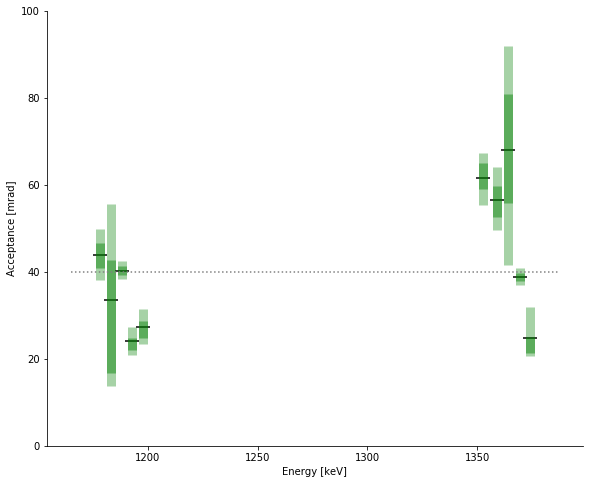
\includegraphics[width=0.8\textwidth]{figures/acceptance_uncertainty.png}}
        \caption[Final acceptances]{Final acceptances for St.\ George
            determined by measuring the \alpa{} yield and comparing to
            the expected value from the beam, target, and cross section
            properties. The \textit{maximum a posterior} acceptance values
            are shown as the black tick marks. The displayed uncertainty bounds are the 67\,\%
            band (dark green) and the 95\,\% band (light green). The
            dotted horizontal line is the 40 mrad designed acceptance
            for St.\ George.}
    \end{center}
\end{figure}

\begin{landscape}
\begin{table}
    \begin{center}
        \caption{ACCEPTANCE WITH UNCERTAINTY}
        \label{tab:acceptance-uncertainty}
        \begin{tabular}{cS[table-format=2.4]S[table-format=3.2]
        S[table-format=3.2]S[table-format=3.2]S[table-format=3.2]
        S[table-format=3.2]S[table-format=3.2]S[table-format=3.2]
        }
            \toprule
            \midrule
            \textbf{Run Number} & \textbf{$E_{\rm p}$ [MeV]} & \textbf{Acceptance [mrad]} &
                \textbf{67\,\%$_{\rm L}$} & \textbf{67\,\%$_{\rm H}$} & \textbf{67\,\%$_{\rm W}$} &
                \textbf{95\,\%$_{\rm L}$} & \textbf{95\,\%$_{\rm H}$} & \textbf{95\,\%$_{\rm W}$} \\
            \midrule
264           & 1.374 & 24.8 & 21.3 & 25.0 &  3.7 & 20.7 & 32.0 & 11.3 \\
270$^\dagger$ & 1.369 & 38.9 & 37.9 & 39.8 &  1.9 & 37.0 & 40.9 &  3.9 \\
277           & 1.364 & 68.1 & 55.7 & 80.9 & 25.2 & 41.5 & 92.0 & 50.6 \\
282           & 1.359 & 56.6 & 52.5 & 59.8 &  7.3 & 49.7 & 64.2 & 14.5 \\
288           & 1.353 & 61.6 & 59.0 & 65.1 &  6.1 & 55.4 & 67.4 & 12.0 \\
248           & 1.198 & 27.3 & 24.8 & 28.7 &  3.8 & 23.4 & 31.5 &  8.2 \\
255           & 1.193 & 24.0 & 21.9 & 24.7 &  2.8 & 21.0 & 27.4 &  6.4 \\
260$^\dagger$ & 1.188 & 40.3 & 39.2 & 41.3 &  2.1 & 38.3 & 42.4 &  4.1 \\
234           & 1.183 & 33.4 & 16.7 & 42.7 & 26.0 & 13.8 & 55.6 & 41.8 \\
241           & 1.178 & 43.8 & 40.9 & 46.7 &  5.8 & 38.2 & 49.9 & 11.7 \\
            \bottomrule
        \end{tabular}

        \vspace{0.5em}
        $\dagger$: Denotes runs at resonance energy
    \end{center}
\end{table}
\end{landscape}

The acceptance values have different uncertainties based on the
specifics of the run, such as the beam energy used and the underlying
cross section. The uncertainty around the on-resonance runs are the
smallest due to the higher count rate, shorter run times, and the
underlying cross section. The cross section peaks for the on-resonance
runs peaks near the center of the energy range covered by the target,
resulting in a slight shift in beam energy having a smaller effect on
the final yield and thus a lower final uncertainty due to the
uncertainty in the beam energy (see
Fig.~\ref{fig:example-cross-section}).

\begin{figure}
    \begin{center}
        \label{fig:example-cross-section}
        \centerline{
            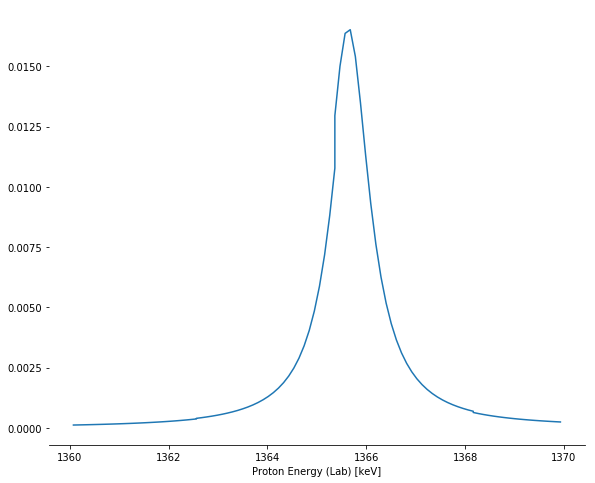
\includegraphics[width=0.8\textwidth]{figures/xs_example.png}}
        \caption[Example cross section]{Example cross section for a run
            near the resonance energy. Note that the scale is linear. As
            the cross section peak is near the center of the energy range
            that the beam has within the target, the final yield is not
            drastically affected by the uncertainty in the beam energy.}
    \end{center}
\end{figure}

From our analysis, we can also decompose the uncertainty for each run
into the contributions from individual uncertainties through our Monte
Carlo method. By focusing in the four uncertainties that are primarily
under the control of the experimenter\---{}the beam energy uncertainty
$E_{\rm beam}$, the run time uncertainty $t_{\rm run}$, the beam current
uncertainty $i_{\rm beam}$, and the target thickness uncertainty
$\Delta_{rm target}$\---{}the focus of subsequent experiments can be on
minimizing the largest uncertainty where necessary. The contributions
ofthe uncertainties are shown in
Tables~\ref{tab:acceptance-uncertainty-67} and
\ref{tab:acceptance-uncertainty-95}, where the values are the percentage
of the 67\,\% and the 95\,\% (respectively) confidence intervals that
remains when holding the given variable or variables constant.

\begin{landscape}
\begin{longtable}
    \begin{center}
        \caption{ACCEPTANCE BOUNDS WITH HELD VARIABLES, 67\,\%}
        \label{tab:acceptance-uncertainty-67}
        \begin{tabular}{cS[table-format=4.2]S[table-format=4.2]S[table-format=4.2]S[table-format=4.2]
        S[table-format=4.2]S[table-format=4.2]S[table-format=4.2]S[table-format=4.2]S[table-format=4.2]S[table-format=4.2]
        }
            \toprule
            \midrule
            \textbf{Held Variables} &
                \textbf{1.178 MeV} & \textbf{1.183 MeV} & \textbf{1.188 MeV}$^\dagger$ & \textbf{1.193 MeV} & \textbf{1.198 MeV} &
                \textbf{1.353 MeV} & \textbf{1.359 MeV} & \textbf{1.364 MeV} & \textbf{1.369 MeV}$^\dagger$ & \textbf{1.374 MeV} \\
            \midrule
$E_{\rm beam}$
    &  49.0 &   5.8 &  96.0 &  92.1 &  95.7 &  64.2 &  37.8 &  13.8 & 106.2 &  68.8 \\
$t_{\rm run}$
    & 101.4 &  93.5 &  98.3 & 103.3 & 101.8 &  97.4 & 101.4 & 100.2 & 105.0 &  99.2 \\
$i_{\rm beam}$
    &  90.7 &  96.1 &  24.7 &  29.3 &  61.1 &  78.1 &  90.8 & 101.9 &  27.0 &  87.4 \\
$\Delta_{\rm target}$
    & 102.1 &  96.1 &  99.6 &  95.9 &  82.2 &  99.3 &  99.9 &  99.5 & 105.9 &  85.6 \\
$E_{\rm beam}$, $t_{\rm run}$
    &  51.0 &   5.9 &  97.8 &  89.5 &  92.5 &  62.9 &  38.3 &  13.3 & 101.3 &  66.7 \\
$E_{\rm beam}$, $i_{\rm beam}$
    &  12.8 &   1.3 &  23.5 &  20.2 &  56.1 &  19.5 &  12.3 &   3.2 &  24.3 &  57.8 \\
$E_{\rm beam}$, $\Delta_{\rm target}$
    &  49.0 &   5.8 &  97.8 &  88.9 &  76.7 &  59.0 &  37.5 &  13.6 & 101.3 &  31.1 \\
$t_{\rm run}$, $i_{\rm beam}$
    &  92.3 &  99.7 &  11.4 &  23.3 &  63.0 &  75.9 &  92.0 & 100.0 &  12.5 &  87.2 \\
$t_{\rm run}$, $\Delta_{\rm target}$
    & 101.8 &  94.7 &  98.1 &  98.4 &  80.3 &  91.9 &  98.2 &  98.6 & 102.7 &  83.2 \\
$i_{\rm beam}$, $\Delta_{\rm target}$
    &  88.9 &  98.8 &  25.2 &  22.4 &  24.1 &  76.1 &  92.6 &  98.9 &  26.1 &  77.1 \\
$E_{\rm beam}$, $t_{\rm run}$, $i_{\rm beam}$
    &  11.2 &   0.8 &   7.8 &  17.4 &  56.0 &  18.9 &  11.4 &   1.3 &   5.4 &  58.2 \\
$E_{\rm beam}$, $t_{\rm run}$, $\Delta_{\rm target}$
    &  49.8 &   5.8 &  95.7 &  88.4 &  76.5 &  58.8 &  37.7 &  13.3 &  98.8 &  29.0 \\
$E_{\rm beam}$, $i_{\rm beam}$, $\Delta_{\rm target}$
    &   7.8 &   1.3 &  21.3 &  10.1 &   5.0 &   8.5 &   7.1 &   2.8 &  22.8 &   6.6 \\
$t_{\rm run}$, $i_{\rm beam}$, $\Delta_{\rm target}$
    &  89.4 &  99.6 &  10.9 &  17.9 &  21.5 &  78.6 &  93.4 & 102.3 &  10.9 &  76.2 \\
All
    &   5.6 &   0.7 &   3.9 &   3.6 &   3.8 &   6.4 &   5.0 &   0.9 &   3.9 &   2.0 \\
            \bottomrule
        \end{tabular}

        \vspace{0.5em}
        $\dagger$: Denotes runs at resonance energy
    \end{center}
\end{longtable}
\end{landscape}

\begin{landscape}
\begin{table}
    \begin{center}
        \caption{ACCEPTANCE BOUNDS WITH HELD VARIABLES, 95\,\%}
        \label{tab:acceptance-uncertainty-95}
        \begin{tabular}{cS[table-format=4.2]S[table-format=4.2]S[table-format=4.2]S[table-format=4.2]
        S[table-format=4.2]S[table-format=4.2]S[table-format=4.2]S[table-format=4.2]S[table-format=4.2]S[table-format=4.2]
        }
            \toprule
            \midrule
            \textbf{Held Variables} &
                \textbf{1.178 MeV} & \textbf{1.183 MeV} & \textbf{1.188 MeV}$^\dagger$ & \textbf{1.193 MeV} & \textbf{1.198 MeV} &
                \textbf{1.353 MeV} & \textbf{1.359 MeV} & \textbf{1.364 MeV} & \textbf{1.369 MeV}$^\dagger$ & \textbf{1.374 MeV} \\
            \midrule
$E_{\rm beam}$
    &  49.4 &   7.5 & 101.1 &  75.8 &  93.0 &  64.1 &  39.6 &  13.2 & 102.4 &  50.9 \\
$t_{\rm run}$
    & 101.8 &  95.3 & 101.3 &  99.8 &  99.6 & 102.7 & 101.0 &  97.9 &  99.0 & 107.6 \\
$i_{\rm beam}$
    &  86.6 &  97.3 &  26.8 &  51.1 &  66.3 &  77.7 &  93.9 &  93.6 &  26.5 & 102.0 \\
$\Delta_{\rm target}$
    &  95.4 &  98.2 & 101.4 &  80.4 &  82.9 &  98.7 & 104.2 &  95.8 & 103.5 &  75.8 \\
$E_{\rm beam}$, $t_{\rm run}$
    &  47.4 &   7.2 &  96.7 &  73.4 &  93.4 &  63.8 &  39.6 &  13.2 & 101.4 &  50.2 \\
$E_{\rm beam}$, $i_{\rm beam}$
    &  12.0 &   1.7 &  23.0 &  18.1 &  55.5 &  20.1 &  12.5 &   3.0 &  24.0 &  42.7 \\
$E_{\rm beam}$, $\Delta_{\rm target}$
    &  46.8 &   7.6 & 100.3 &  72.0 &  73.8 &  60.4 &  38.0 &  12.9 & 103.5 &  20.6 \\
$t_{\rm run}$, $i_{\rm beam}$
    &  88.0 &  97.2 &  13.4 &  50.1 &  64.6 &  78.2 &  96.8 &  96.9 &  15.2 &  94.7 \\
$t_{\rm run}$, $\Delta_{\rm target}$
    &  98.5 &  98.3 &  98.2 &  86.7 &  83.5 &  99.4 & 102.0 &  98.8 &  99.8 &  75.9 \\
$i_{\rm beam}$, $\Delta_{\rm target}$
    &  87.7 &  95.9 &  26.6 &  29.7 &  29.1 &  76.9 &  93.4 &  93.5 &  25.6 &  72.9 \\
$E_{\rm beam}$, $t_{\rm run}$, $i_{\rm beam}$
    &  11.1 &   1.0 &   8.1 &  18.6 &  54.0 &  17.8 &  11.5 &   1.5 &   8.3 &  43.5 \\
$E_{\rm beam}$, $t_{\rm run}$, $\Delta_{\rm target}$
    &  47.4 &   7.2 &  96.8 &  70.1 &  76.0 &  59.9 &  39.0 &  12.9 &  99.4 &  20.4 \\
$E_{\rm beam}$, $i_{\rm beam}$, $\Delta_{\rm target}$
    &   7.9 &   1.6 &  21.4 &   8.4 &   5.0 &   8.4 &   7.4 &   2.7 &  22.4 &   4.6 \\
$t_{\rm run}$, $i_{\rm beam}$, $\Delta_{\rm target}$
    &  86.2 &  98.6 &  13.1 &  29.6 &  27.0 &  78.2 &  94.2 &  96.5 &  14.5 &  68.0 \\
All
    &   5.4 &   1.0 &   4.0 &   2.8 &   3.8 &   6.6 &   5.2 &   0.9 &   3.7 &   1.3 \\
            \bottomrule
        \end{tabular}

        \vspace{0.5em}
        $\dagger$: Denotes runs at resonance energy
    \end{center}
\end{table}
\end{landscape}

Since the final contributions to the uncertainty are not known, and the
correlations between different variables not explicitly taken into
account, these values should be used as a guide instead of for their
absolute values. From the above tables, we can make generalizations
about which uncertainties may have the largest impact on further
studies. The on-resonance runs are extremely dependent on the beam
current uncertainty, as the beam current directly affects what the final
yield at the detector will be, and if a smaller uncertainty band is
required, controlling the beam current and reducing its uncertainty
should be the most important aspect of the experiment. Conversely, the
point just below the resonance in energy has an extremely large final
uncertainty, mainly due to the beam energy uncertainty. Due to the
nature of the cross section, a small shift in beam energy can result in
drastically different final yields due to the rapidly changing cross
section below the resonance. Subsequent below-resonance runs should
focus on reducing the uncertainty from the beam energy, which requires
spending more time fine-tuning the accelerator to provide a more
energy-stable beam to the experimental area.

Additionally, the complete uncertainty for our acceptance values cannot
be reduced to zero. The irreducible uncertainty present (in the last row
of Tables~\ref{tab:acceptance-uncertainty-67} and
\ref{tab:acceptance-uncertainty-95}) for each run is from the
uncertainties due to SRIM, the detector statistics, and other sources
as described in Section~\ref{sec:uncertainties}.


\section{Advantages and Disadvantages}
% from call with Manoel: 2018-05-16
(p,a) can suffer from elastic scattering, but St. George can avoid that
by looking at zero degrees. Ratio of alphas to elastically scattered
protons can have a prohibitivve count rate

Disadvantage: no angular distribution, requires recoil separator
Advantage: can avoid killing detectors, check zero degree


\section{Uncertainties}
\label{sec:uncertainties}

The final uncertainties on the acceptances at each run energy are skewed
distributions. Since basic error propagation relies on the errors being
gaussian distributed, the fact that our uncertainties are not partially
justifies the Bayesian approach described previously. Part of the reason
for the skewed distributions is that the acceptance is bounded by zero
and $\pi/2$, and since our distributions sit closer to the zero end
instead of near the middle of the range somewhat requires that the
distribution be skewed. Our process avoids propagating errors from
arbitrary or non-Gaussian distributions and allows for a richer
discussion of the contributions of each uncertainty.

\subsection{Statistical}

The uncertainties on most of the inputs can be considered to be gaussian distributed, as
that represents the statistical nature of the process that creates that
input value. Individual collections of these values still exhibit a
normal distribution. For values that may be extremely skewed on are
known to have other properties, a gaussian distribution may not be the
correct underlying uncertainty for the value.

Our final acceptance measurement has a skewed distribution, which can be
evidenced from the fact that the angular acceptance cannot be a negative
value. In this case, if we were to directly model the final uncertainty
of our acceptance, a log-normal distribution would be more apt. For each
uncertainty, a brief description of the underlying assumptions will be
presented.

\textbf{Target thickness:} no assumed underlying distribution. The target
thickness measurements performed before the experiment were used to
determine the particle density within the target. The counts at the
detector for the runs were assumed to be Poisson distributed since they
are discrete counts. From the peak shifts due to energy loss when the
$\alpha$ particles passed through the target, the number of target nuclei
could be determined. The original spectra were used as the base properties
to generate new count distributions, each of which when combined with the
energy loss would lead to a unique number of target nuclei. The SRIM
tabulated values that were used to relate the energy loss through the
target to the target thickness were assumed to have a gaussian distribution,
where the standard deviation was taken as 3\,\% of the nominal value. For subsequent
uses of the target thickness, a number was drawn from the generated distribution.
If a model for the target thickness were desired, the shape was approximately
Gaussian with parameters $\mu = 1.42$ and $\sigma = 0.03$ ($\times 10^{18}$
nuclei/cm\squared{}).

\textbf{Beam energy:} gaussian distributed. The underlying statistical
fluctuation of the multiple additive and multiplicative values that
determine the beam energy\---{}the power supplies for the ion source,
accelerator, and analyzing magnet\---{}result in a gaussian distribution
for the beam energy. While the beam energy can never be negative and thus
may be better modeled by a log-normal distribution, the values of the beam
energy are sufficiently far from zero such that the assumption of a normal
distribution can be used. The mean of the distribution is based on the setpoint
for the run, which the standard deviation is constant for all runs. A
value of 500~eV was taken as a conservative value from previous energy
calibration runs. Since no explicit energy calibration was performed
using the exact setup for this experiment, this conservative value
represents that additional uncertainty.

\textbf{Beam current:} gaussian distributed. For similar reasons as the
beam energy uncertainty, a gaussian distribution for the beam current
was chosen. Observations on the beam current roughly showed a normal
distribution around a central value, and the values and fluctuation were
such that a log-normal distribution did not need to be assumed. During
experimental runs, samples of the beam current were taken. Without a direct
measurement of the beam current during the run, which could be obtained
using an offset Faraday cup or Si detector, no more information about the
beam current could be obtained. A cauchy distribution may be considered
as an alternative, especially when the accelerator system is producing
extremely variable currents, due to the heavier tails of the distribution.
For our pruposes, conservative estimates of the beam current were obtained
from a gaussian distribution based on the current observations performed
during the experiment and shown in Table~\ref{tab:beam-current-uncertainty}.

\begin{table}
    \begin{center}
        \caption{BEAM CURRENT UNCERTAINTY}
        \label{tab:beam-current-uncertainty}
        \begin{tabular}{cS[table-format=4.2]S[table-format=4.2]S[table-format=4.2]}
            \toprule
            \midrule
            \textbf{Run} & \textbf{$E_{\rm p}$ [MeV]} & \textbf{$i_{\rm p}$ [$\mu$A]} &
                \textbf{$\delta i_{\rm p}$ [$\mu$A]} \\
            \midrule
                264           & 1.374 & 2.75 & 0.14 \\
                270$^\dagger$ & 1.369 & 2.60 & 0.13 \\
                277           & 1.364 & 2.70 & 0.14 \\
                282           & 1.359 & 2.50 & 0.13 \\
                288           & 1.353 & 2.34 & 0.15 \\
                248           & 1.198 & 2.18 & 0.24 \\
                255           & 1.193 & 1.85 & 0.19 \\
                260$^\dagger$ & 1.188 & 2.50 & 0.13 \\
                234           & 1.183 & 2.00 & 0.10 \\
                241           & 1.178 & 2.47 & 0.16 \\
            \bottomrule
        \end{tabular}

        \vspace{0.5em}
        $\dagger$: Denotes runs at resonance energy
    \end{center}
\end{table}

\textbf{Time:} gaussian distribution. Our run times were recorded both
as a coarse clock time for the start and end of the run and with the DAQ.
For those runs lasting longer than 15 minutes, additional stopages in the
measurement were made in the middle of the run without stopping the DAQ.
Values recorded by the DAQ also differed from the set values for the total
run time. As each of these factors has a role in the total run time of
the experiment and are approximately additive in nature, a gaussian
distribution makes sense here. The longer runs had both the stopage time
estimated and subtracted from the total run time, and the uncertainty was
also taken to be larger. The uncertainties for the run time are given
in Table~\ref{tab:run-time-uncertainty}.

\begin{table}
    \begin{center}
        \caption{RUN TIME UNCERTAINTY}
        \label{tab:run-time-uncertainty}
        \begin{tabular}{cS[table-format=2.4]S[table-format=5]S[table-format=3]}
            \toprule
            \midrule
            \textbf{Run} & \textbf{$E_{\rm p}$ [MeV]} & \textbf{$t$ [s]} &
                \textbf{$\delta t$ [s]} \\
            \midrule
                264           & 1.374 &  910 & 10 \\
                270$^\dagger$ & 1.369 &  906 & 10 \\
                277           & 1.364 &  989 & 10 \\
                282           & 1.359 & 3182 & 22 \\
                288           & 1.353 & 9436 & 53 \\
                248           & 1.198 & 5455 & 26 \\
                255           & 1.193 &  907 & 10 \\
                260$^\dagger$ & 1.188 &  907 & 10 \\
                234           & 1.183 & 1078 & 10 \\
                241           & 1.178 & 6503 & 51 \\
            \bottomrule
        \end{tabular}

        \vspace{0.5em}
        $\dagger$: Denotes runs at resonance energy
    \end{center}
\end{table}

\textbf{Detector counts:} Poisson distribution. As each bin within the
Si detector spectra counts the particles that fall within that energy
bucket, a Poisson distribution was adopted for the detector counts. This
choice is common for counting experiments.

\textbf{SRIM tabulated values:} gaussian distribution. The target stopping
power and those values related to finding the target thickness were taken
from SRIM. Due to the fact that the \alpa{} reaction is relativvely well
studied, a conservative estimate of 3\,\% was adopted for all values
arising from SRIM results.

The final uncertainty bands for each of the acceptance measurements can
be analyzed by what values affect the range for the uncertainty. We can
limit this discussion to inputs that are controllable by the
experimenter. The final uncertainty will be made up of the uncertainty
from inputs and the uncertainty from those statistical and irreducible
processes. The four inputs that the experimenter can control are the
energy, time, current, and thickness uncertainties. The energy
uncertainty is related to the stability of the accelerator and the
calibration of the analyzing magnet, both of which can be measured and
regulated to the point where the uncertainty can be minimized. The time
uncertainty is based on the total runtime and the interruptions caused
by requiring the stoppage of the beam in order to measure the current
and can be reduced through synchronization of the DAQ with the start of
bombardment, and by minimizing interruptions during the data collection
process. The current uncertainty can be minimized by measuring the
current continuously during the experiment, as there will then be fewer
unknown changes in the beam current and a single value for the beam
current does not need to be applied to the entirety of the experimental
run. Finally, the thickness uncertainty can be minimized by performing
target thickness measurements at multiple energies and with potentially
multiple particles, and by running those measurements for longer such
that the energy loss by the particles can be more accurately determined.

Each of these inputs affects a different part of the final acceptance,
based on how it relates to the experimental and theoretical yield, or
both. We can determine the impact of reducing the uncertainty on each of
these inputs by setting the uncertainty to zero within the analysis
pipeline, which would return a different uncertainty band for the run in
question. Since these uncertainties are not necessarily independent of
each other, we should also look at all combinations of these four inputs
being controlled for to get a full picture of the impartances.
Additionally, the irreducible uncertainty can be determined by keeping
all of the inputs constant. The contribution to the final uncertainty is
expressed as a percent of the total uncertainty band for both the 67\,\%
and 95\,\% confidence interval, so the amount of the band that is
accounted for by the inputs that are not held constant.

\subsection{Systematic}

%% NOTES

systematic: alphas hitting interior walls, energy cutoff at detector,
transmission (faraday cup offset?)

Missed counts can be measured, say that target cup roughly restricts to
40 mrad in all directions, so those additional counts could be from
within 40 mrad (I feel weird about this, so don't directly add it in,
but mention the amounts either here or in potential sources of error)

%% END NOTES

Potential sources of systematic uncertainty must also be considered when
discussing the acceptance results. As low yield future experiments would
not have the relatively high count rates at the detector seen during this
experiment, the potential for lost counts due to the systematics could
drastically affect the final yield and thus the cross section measurements.
Potential sources of systematic uncertainty can be divided into experimental
sources and analytical sources.




\section{Uniformity of Acceptances}
\label{sec:uniformity-of-acceptances}

When calculating the acceptance for St.\ George, it was assumed that the
acceptance cone was described by a single opening angle. In practice,
the horizontal and vertical opening angles may be distinct from each
other. During preliminary experiments for the acceptance of St.\ George,
it required much less fine tuning of magnetic fields to achieve the
maximum vertical acceptance than it was to achieve the maximum
horizontal acceptance. This observation may be due to the lack of
dispersive elements in the vertical plane.

The strips of the Si detector were aligned such that an individual strip
was oriented in the vertical direction, or a particle that is deflected
horizontally would be detected on a different strip (see FIGURE). This
orientation allowed for improved tuning in the horizontal plane with the
lack of sensitivity in the vertical plane. The auxiliary runs performed
where the detector was place in the ``low'' position (where the top of
the detector is located where the bottom of the detector would be in the
regular running position) inform the amount of particles that are not
captured in the vertical plane due to minor mistuning of the separator,
and the auxiliary runs used to center the produced alpha particle
distribution on the detector horizontally inform the amount of particles
that are not captured in the horizontal direction. Ideally, a detector
segmented in both the horizontal and vertical plane would give a full
description of the alpha-particle beam spot density at the detector
plane and could be used to better relate the distribution of counts at
the detector plane to the acceptance cone at the target location.

In the final configuration of the target system, a series of conical
collimators will be located following the target location to defined the
40 mrad acceptance cone. As the desired configuration of St.\ George is
to measure $(\alpha,\gamma)$ reactions where the heavy recoil particles
are emitted from the target within a cone with an opening angle less
than 40~mrad, the potential effect of a non-symmetric acceptance is reduced.
For experiments similar to this where the ejected
particles are emitted within a cone larger than 40~mrad, these
collimators would ensure that the particles reaching the final detector
must have been emitted within that known acceptance cone. This
restriction would improve the tuning of the separator for similar
experiments, as the emitted particle beam spot at the detector plane can
be more easily tuned to fit completely on the detector.


% \section{Potential Sources of Error}
% \label{sec:potential-sources-of-error}

% The preliminary tunes were determined by keeping a beam with a given
% energy and angular deviation from the mean reached the detector plane
% within the physical space of the detector as measured on a quartz.


\section{The $({\rm p},\alpha_1)$ channel}
\label{sec:the-palpha_1-channel}

At the resonances probed, the $({\rm p},\alpha_1)$ reaction channel is
also open. Measuring the cross section for this reaction at the two
desired resonances is a more difficult experiment due to the lower
rigidity of the produced alpha particles due to the lower energy. The
kinematics for this reaction are given in TABLE.

The lower rigidity is still within the design parameters of St.\ George,
but due to the altered tune required to direct the produced alpha
particles to the detector plane has different rejection properties than
the standard tune. As such, the incident proton beam is close enough in
rigidity that the beam may strike the detector. The beam reduction
levels would not be high enough to avoid damaging the Si detector,
preventing the measurement of the cross section without either
additional rejection capabilities or an improvement in the tune.

MORE DETAILS FROM LOGBOOK


\section{Next Steps}
\label{sec:next-steps}

As a further test of the angular acceptance capabilities of St.\ George,
the experiment discusses herein can be repeated by sending the produced
$\alpha$ particles to the final detector plane. The transmission of
these particles through the entirety of the separator would be able to
use the standard ion transport tune for the separator, avoiding the
requirement of determining an additional set of magnetic field
strengths. A test under these conditions would be a verification of the
angular acceptance under similar conditions as will be seen for
$(\alpha,\gamma)$ experiments during the regular operation of the
separator. The required work to determine the correct field settings for
the final third of St.\ George was beyond the scope of this work, but
will be required for any future study using the detection system at the
end of St.\ George.

In cases where the detection system is placed just beyond the Wien
filter at focal plane $F_2$, care must be taken to properly ground and
shield the cables connecting the detector to the DAQ. This experiment
used a suboptimal bias voltage, resulting in additional noise at low
energy and a drastic decrease in detector resolution. These facts
combined prevented the direct identification of the produced $\alpha$
particles and the final rejection of the remaining incident protons such
that an energy threshold was used to discriminate between the two
particles.


\section{Closing Thoughts}
\label{sec:closing-thoughts}

Fully commissioning a recoil separator requires a vast amount of
coordinated resources and time, and is something that would not be
possible without a large and motivated team behind it. The attention to
detail required for each individual magnet setting and the process
through which that megnet is set can only be accomplished through
extreme rigor on the experimental side as well as on the logging and
information dissemination side. A long memory for the experimental
accomplishments and a short memory for the experimental failings is
beneficial to maintain the morale of the team at a point where work can
continue. Lacking in any of these areas can lead to an increase in the
time required to commission a single section of the separator.

Once sections are commissioned, experimental work building off of the
sections that are now experimentally accessible and understood should be
done to ensure that the understanding of that section is accurate and to
provide an avenue for data analysis for the experimenters involved, both
to maintain morale and to provide for the possibility of publishing
incremental improvements. This experimental work is the outcome of
including these experimental ``checkpoints'' into the grander
commissioning work required for St.\ George, and should be included as
the additional components of the St.\ George system, especially the
addition of the gas target, moving forward.
